\documentclass[a4paper]{article}
\usepackage[margin=3cm]{geometry}
\usepackage[french]{babel}
\usepackage[utf8]{inputenc}
\usepackage{amsmath}
\usepackage{graphicx}
\usepackage{schemabloc}
\usepackage[colorinlistoftodos]{todonotes}
\usepackage{hyperref}
\usepackage{float}

\title{CSE - Asservissement en couple d'un moteur DC}

\author{Corentin Smith - Gabriel Samain}

\date{\today}

\begin{document}
\maketitle


\section{Préambule}

\subsection{Objectif}

L'objectif de ce TP est de réaliser l'asservissement en couple / courant d'un moteur DC, le but final étant de simuler un effort par l'axe du moteur.

\subsection{Théorie}

L'équation électromécanique donne :
$$
C = k \cdot \Phi \cdot I \\
$$

Contrôler le courant dans le moteur revient donc à contrôler le couple.

\section{Boucle d'asservissement}

On réalise une boucle d’asservissement en récupérant l’intensité dans le moteur à l’aide d’une résistance de shunt.

\subsection{Schéma}

\begin{center}
\begin{tikzpicture}
\sbEntree{E}
\sbComp{comp}{E}
\sbRelier[$U_c$]{E}{comp}
\sbBloc{hach}{Hacheur}{comp}
\sbRelier[$\epsilon$]{comp}{hach}
\sbBloc{reg}{Régulateur}{hach}
\sbRelier[$U_h$]{hach}{reg}
\sbBloc{mot}{Moteur}{reg}
\sbRelier[$u$]{reg}{mot}
\sbSortie{S}{mot}
\sbRelier[$I$]{mot}{S}
\sbDecaleNoeudy[4]{S}{E}
\sbBlocr{shunt}{Shunt}{E}
\sbRelieryx{mot-S}{shunt}
\sbBloc{gainshunt}{$K_s$}{E}
\sbRelierxy[$U_s$]{shunt}{gainshunt}
\sbRelierxy[$U_m$]{gainshunt}{comp}
\end{tikzpicture}
\end{center}

\todo{FIXER Schema bloc}

Les blocs assurent les fonctions suivantes :
\begin{description}
  \item[Hacheur] 	Transforme le signal $\epsilon$ en PWM grâce à un comparateur à hysterésis et un signal triangle
  \item[Régulateur] Duplique et inverse le signal précédent puis l'injecte dans un pont en H
  \item[Moteur] 	Le système à contrôler
  \item[Shunt] 		Une résistance de shunt permet de “lire le courant” sous forme de tension
\end{description}

\subsection{Schéma électrique}

La première partie du schéma transforme le signal de commande continu en PWM proportionnel à cette tension.

Le pont en H permet de réaliser une amplification de puissance de la PWM. La tension efficace de cette PWM est proportionnelle à la largeur d'impulsion, et la vitesse de rotation du moteur est donc reliée directement à la tension de commande.

\begin{figure}[H]
\centering
	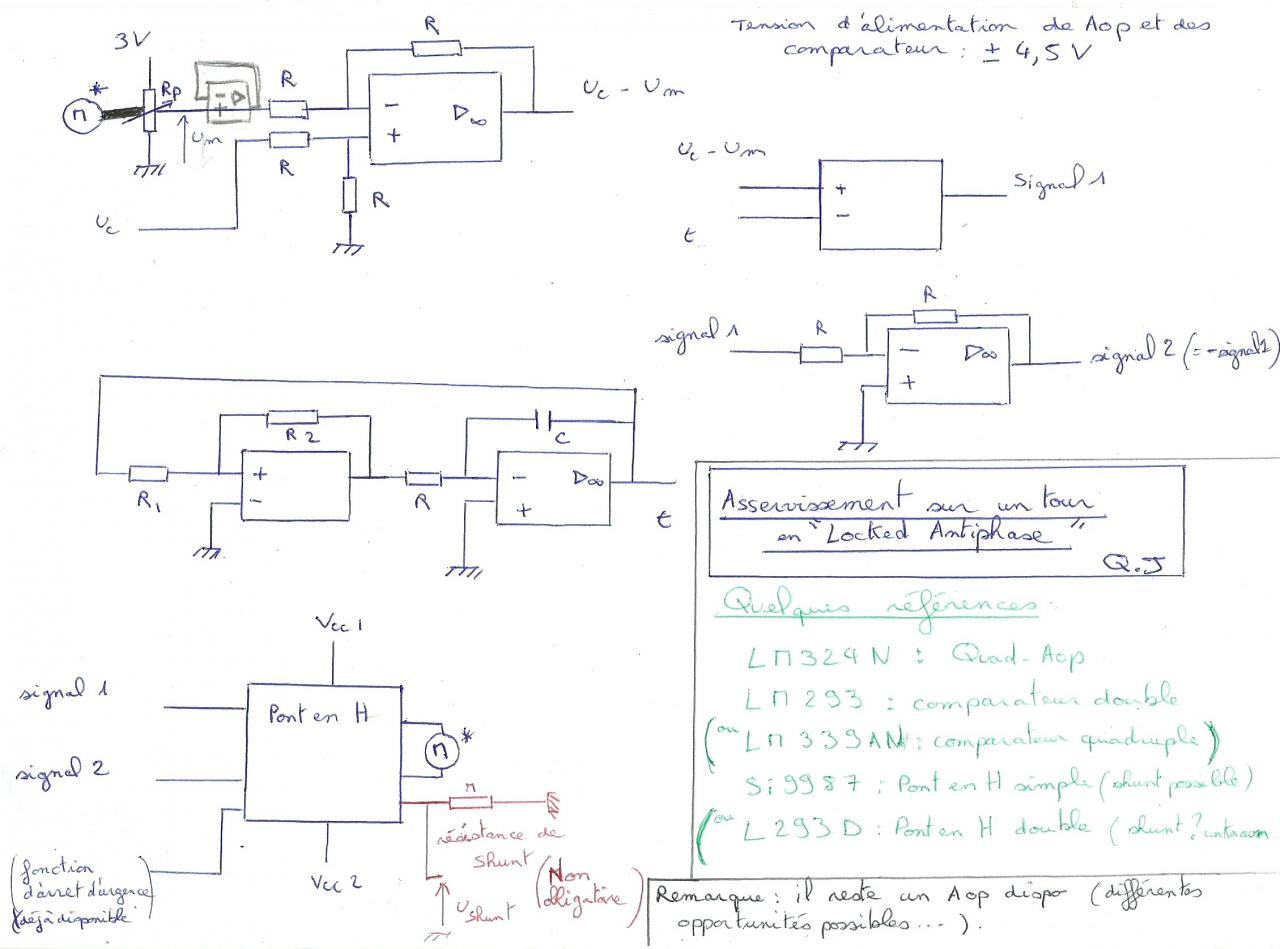
\includegraphics[width=1\textwidth]{schema.png}
	\caption{Schéma électrique en boucle ouverte}
\end{figure}


\begin{figure}[H]
\centering
	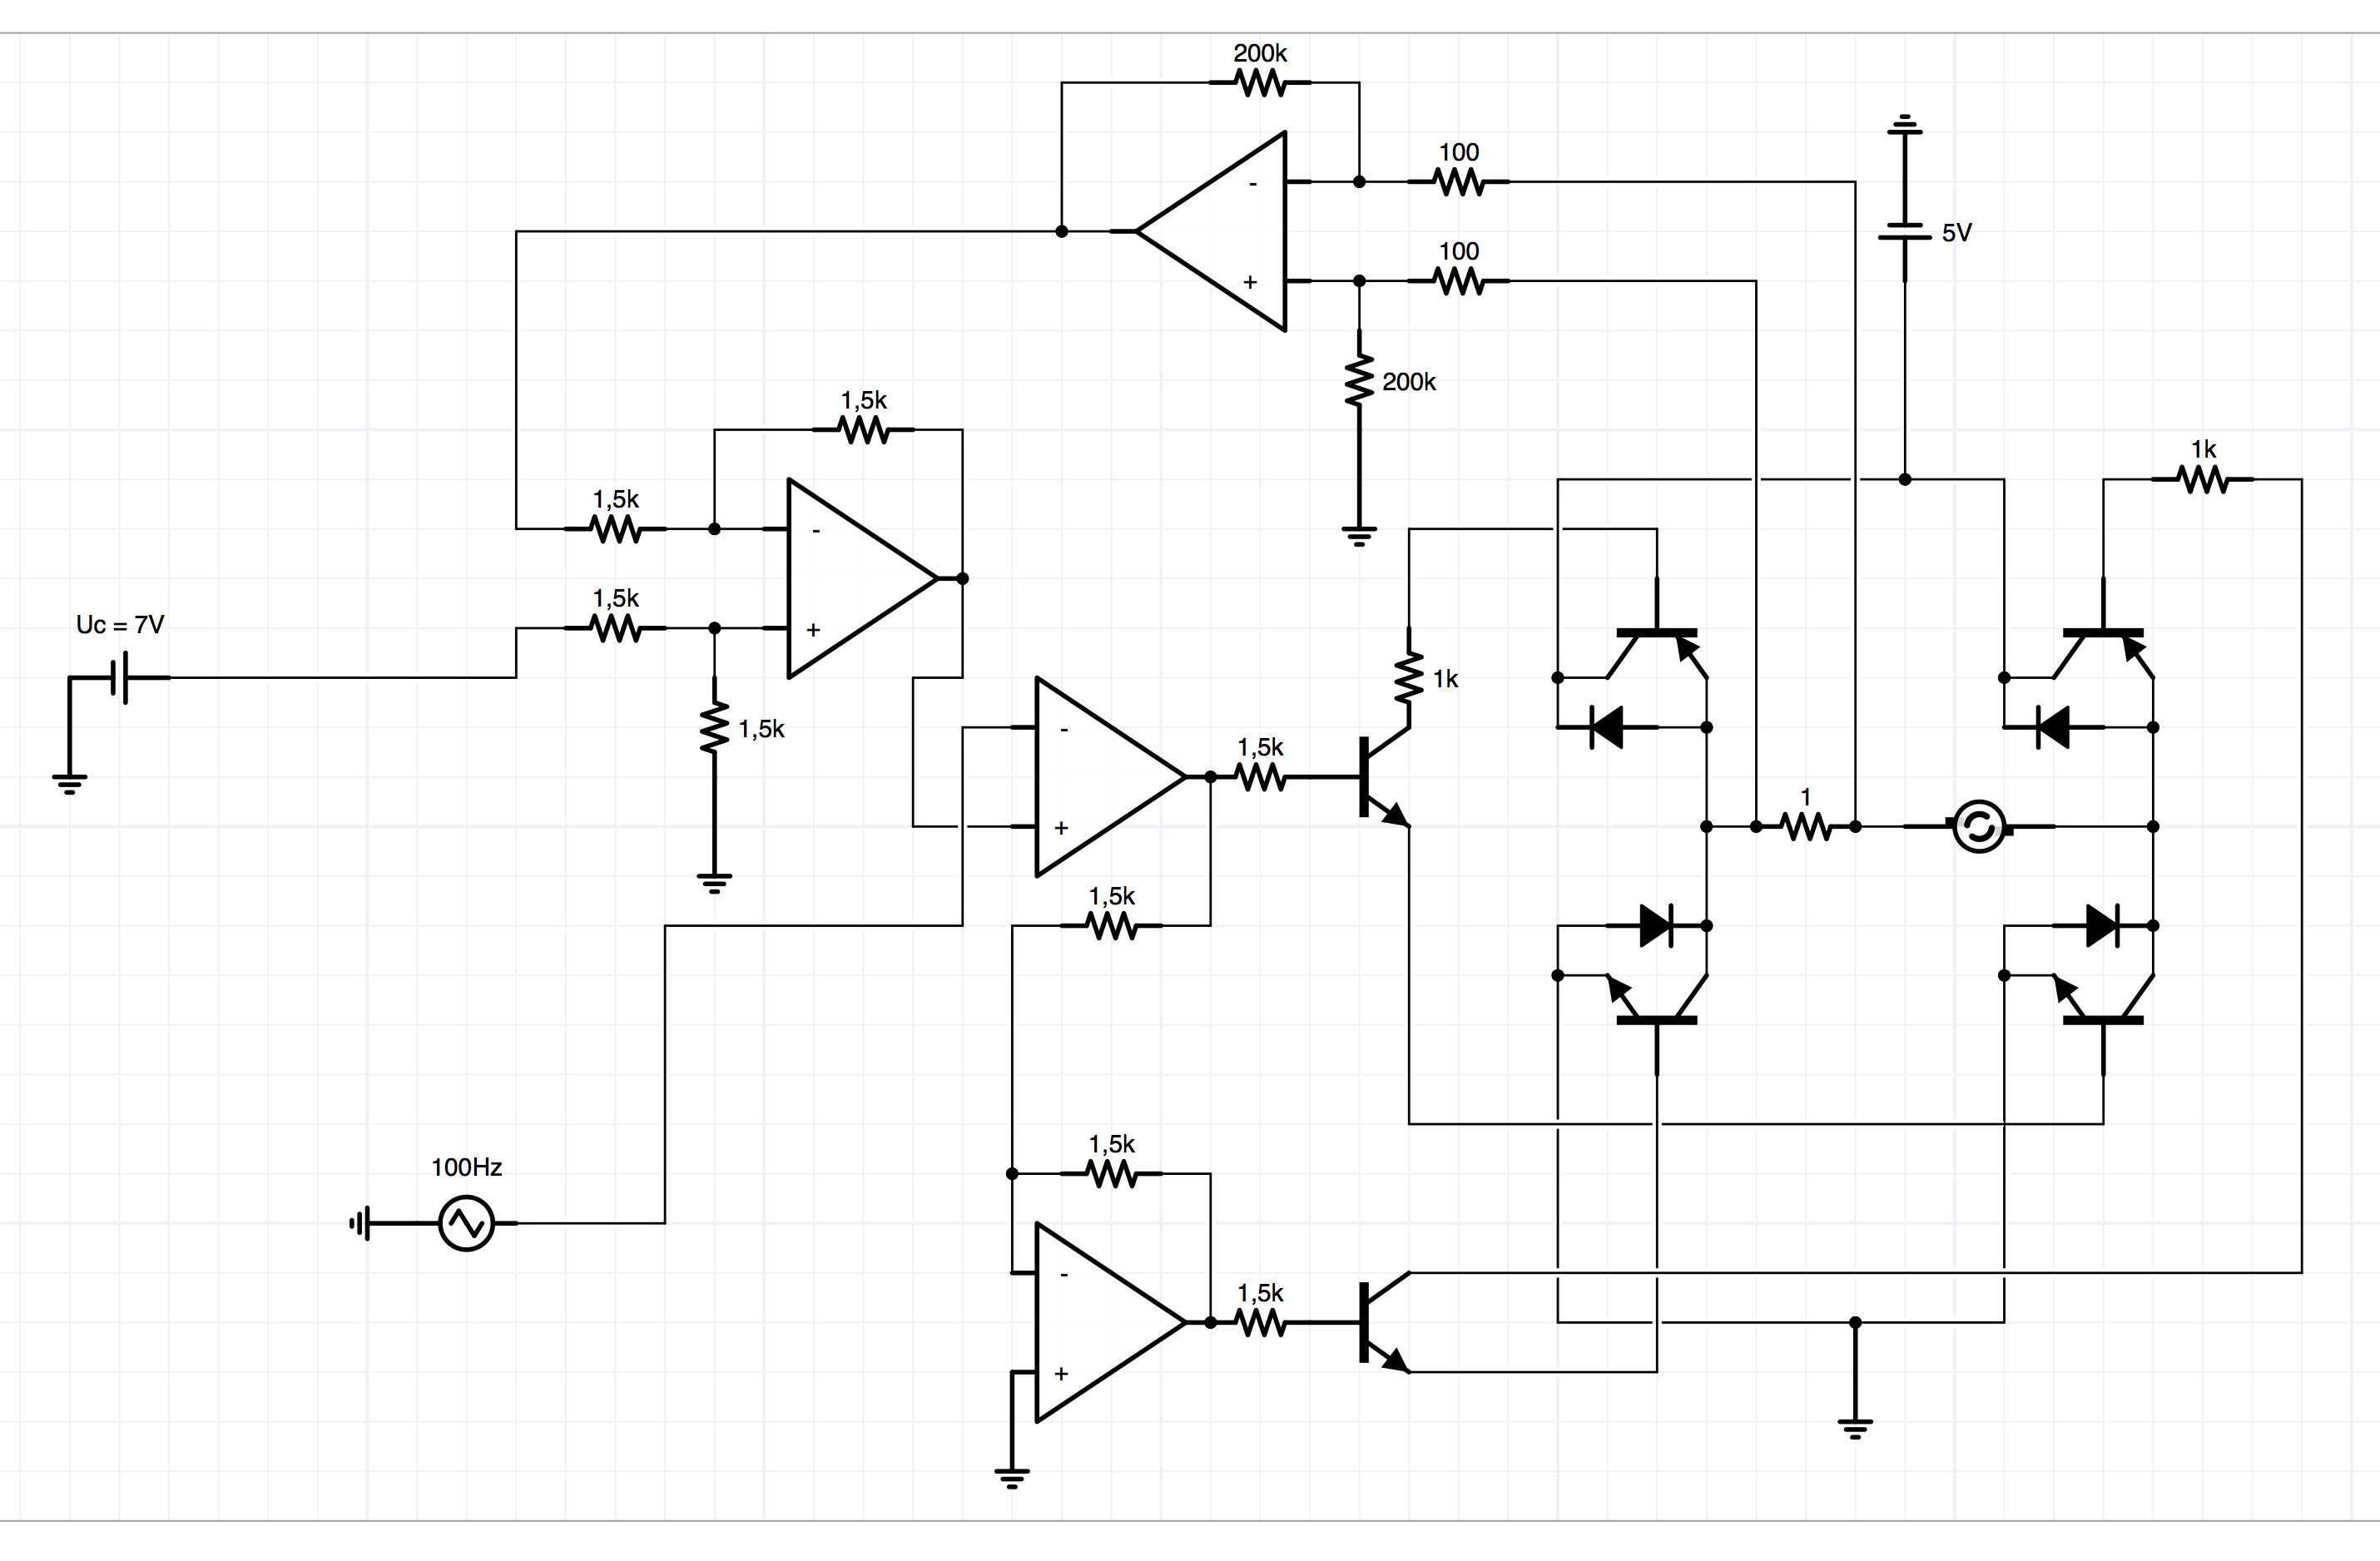
\includegraphics[width=1\textwidth]{schema_boucle.png}
	\caption{Schéma électrique bouclé}
\end{figure}


\subsection{Choix des composants}

Nous avions prévu de réaliser le circuit avec un pont en H de TI, le LMD18245T \href{http://www.ti.com/lit/ds/symlink/lmd18245.pdf}{[datasheet]}, mais nous n'avons pas réussi à le faire fonctionner correctement et nous avons décidé de réaliser le pont en H à la main, le circuit étant assez simple.

Les transistors que nous avons choisis sont des transistors de moyenne puissance, les BD237 (NPN) et BD238 (PNP) \href{http://www.onsemi.com/pub_link/Collateral/BD237-D.PDF}{[datasheet]}.

Les amplificateurs opérationnels sont des LM324AN \href{https://www.fairchildsemi.com/datasheets/LM/LM324.pdf}{[datasheet]}. Nous avons également utilisé les amplificateurs opérationnels en tant que comparateurs afin de limiter le nombre de composants.\\

Afin de déterminer la valeur du gain $K_s$ nécessaire en sortie de la boucle (entre la résistance de shunt et l'entrée du sommateur), nous avons réalisé une série de mesures de la tension aux bornes de la résistance de shunt.

On obtient une courbe bien linéaire qui nous permet de déterminer la valeur de $K_s = 1/0.0166 = 60.24$. On a donc choisi pour les résistances $56k\Omega + 3.9k\Omega$ et $1k\Omega$ pour obtenir un rapport d'environ 60.


\begin{figure}[H]
	\centering
	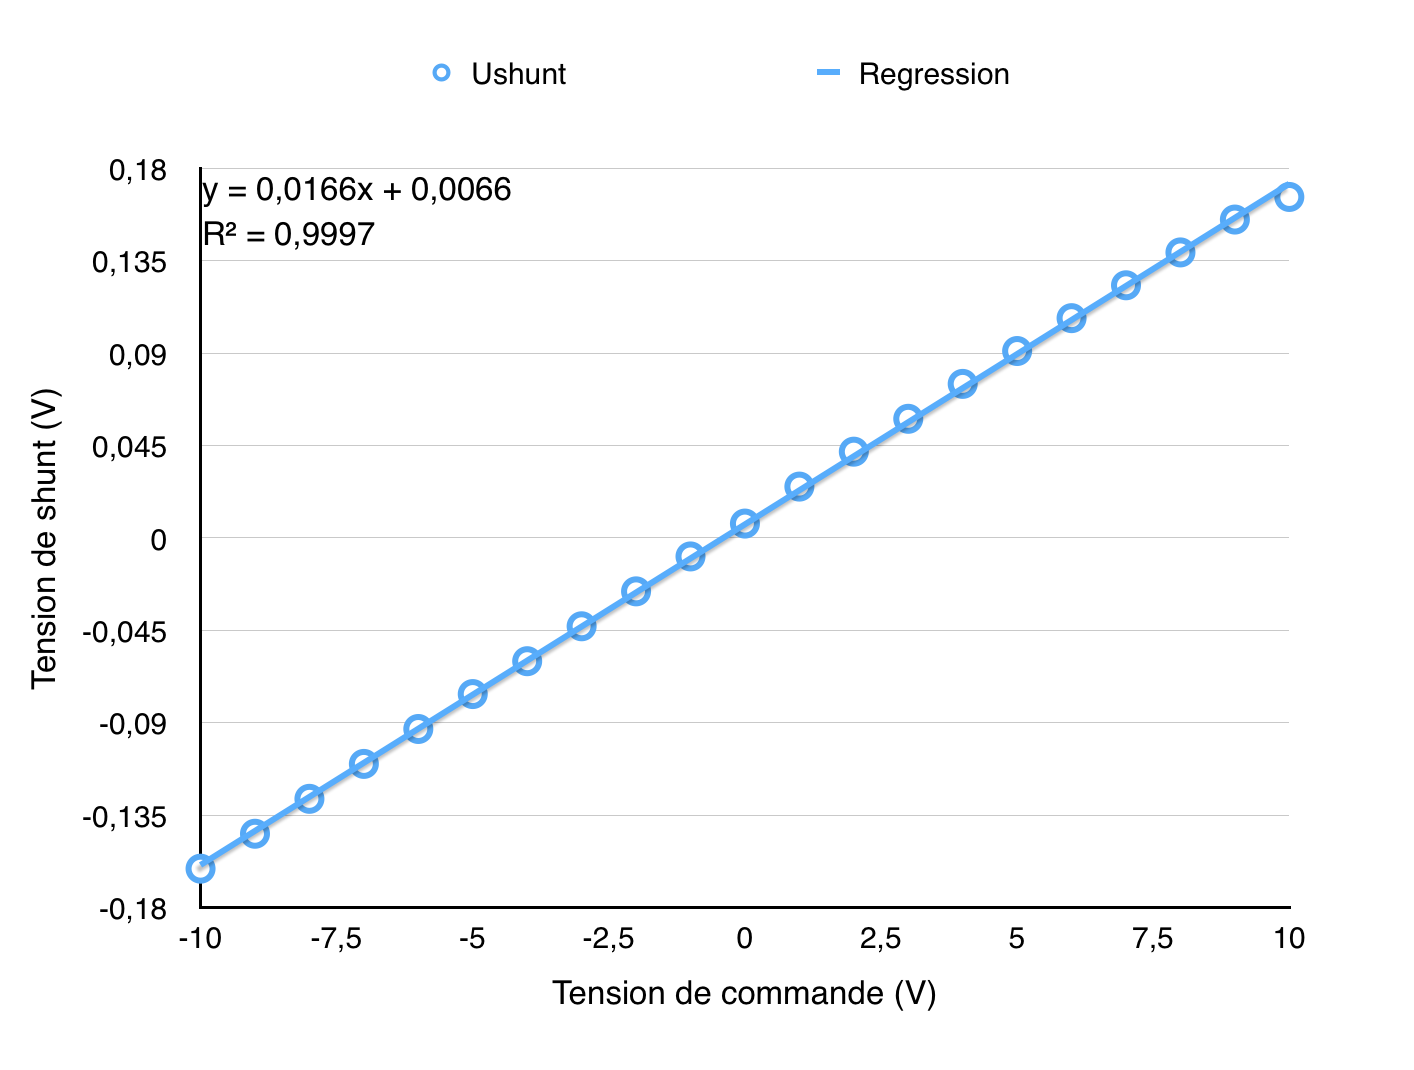
\includegraphics[width=1\textwidth]{graph_shunt.png}
	\caption{Relation entre commande et tension aux bornes de la résistance de shunt}
\end{figure}



\section{Réalisation}

\subsection{Simulation}

La simulation théorique du circuit se fait à l'aide du logiciel iCircuit qui permet une visualisation en temps réel des grandeurs physiques caractéristiques de chaque composant du circuit.

Pour ce qui est du bouclage, le modèle de moteur inclus dans le logiciel n'étant pas très réaliste, nous n'avons pas réalisé de simulation.

\begin{figure}[H]
	\centering
	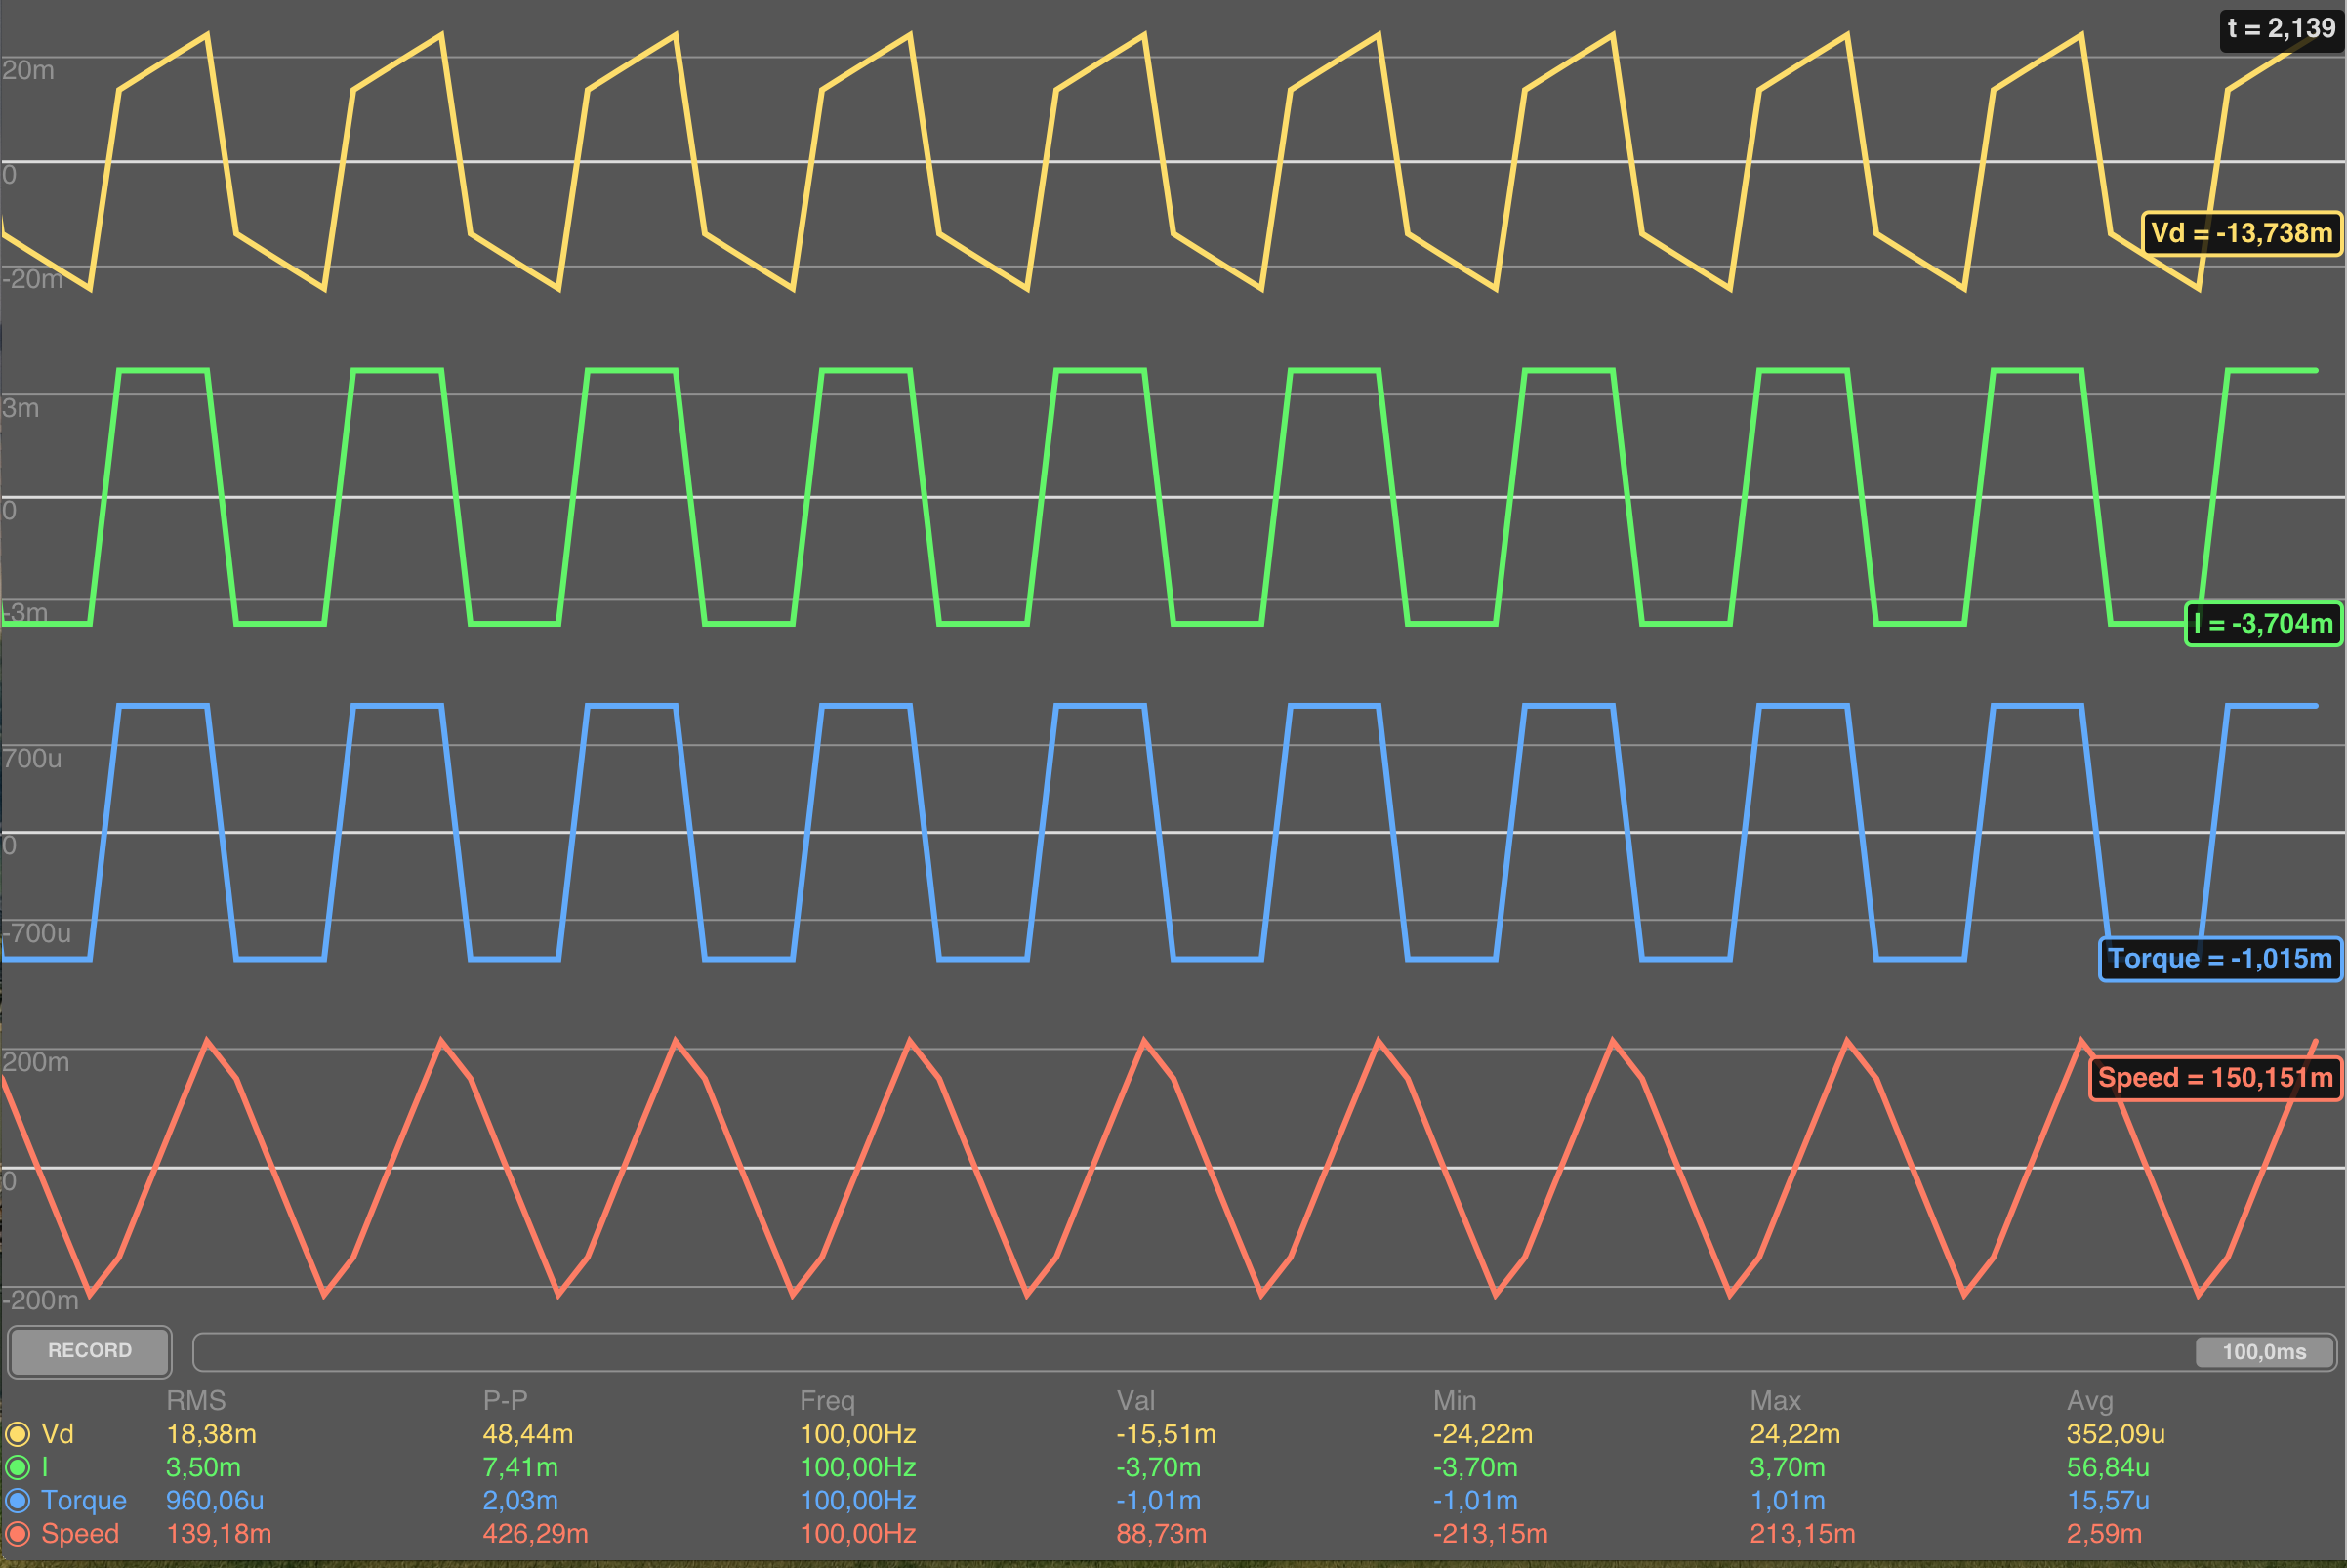
\includegraphics[width=1\textwidth]{simu0v}
	\caption{Simulation (boucle ouverte) avec une commande de 0V}
\end{figure}
\begin{figure}[H]
	\centering
	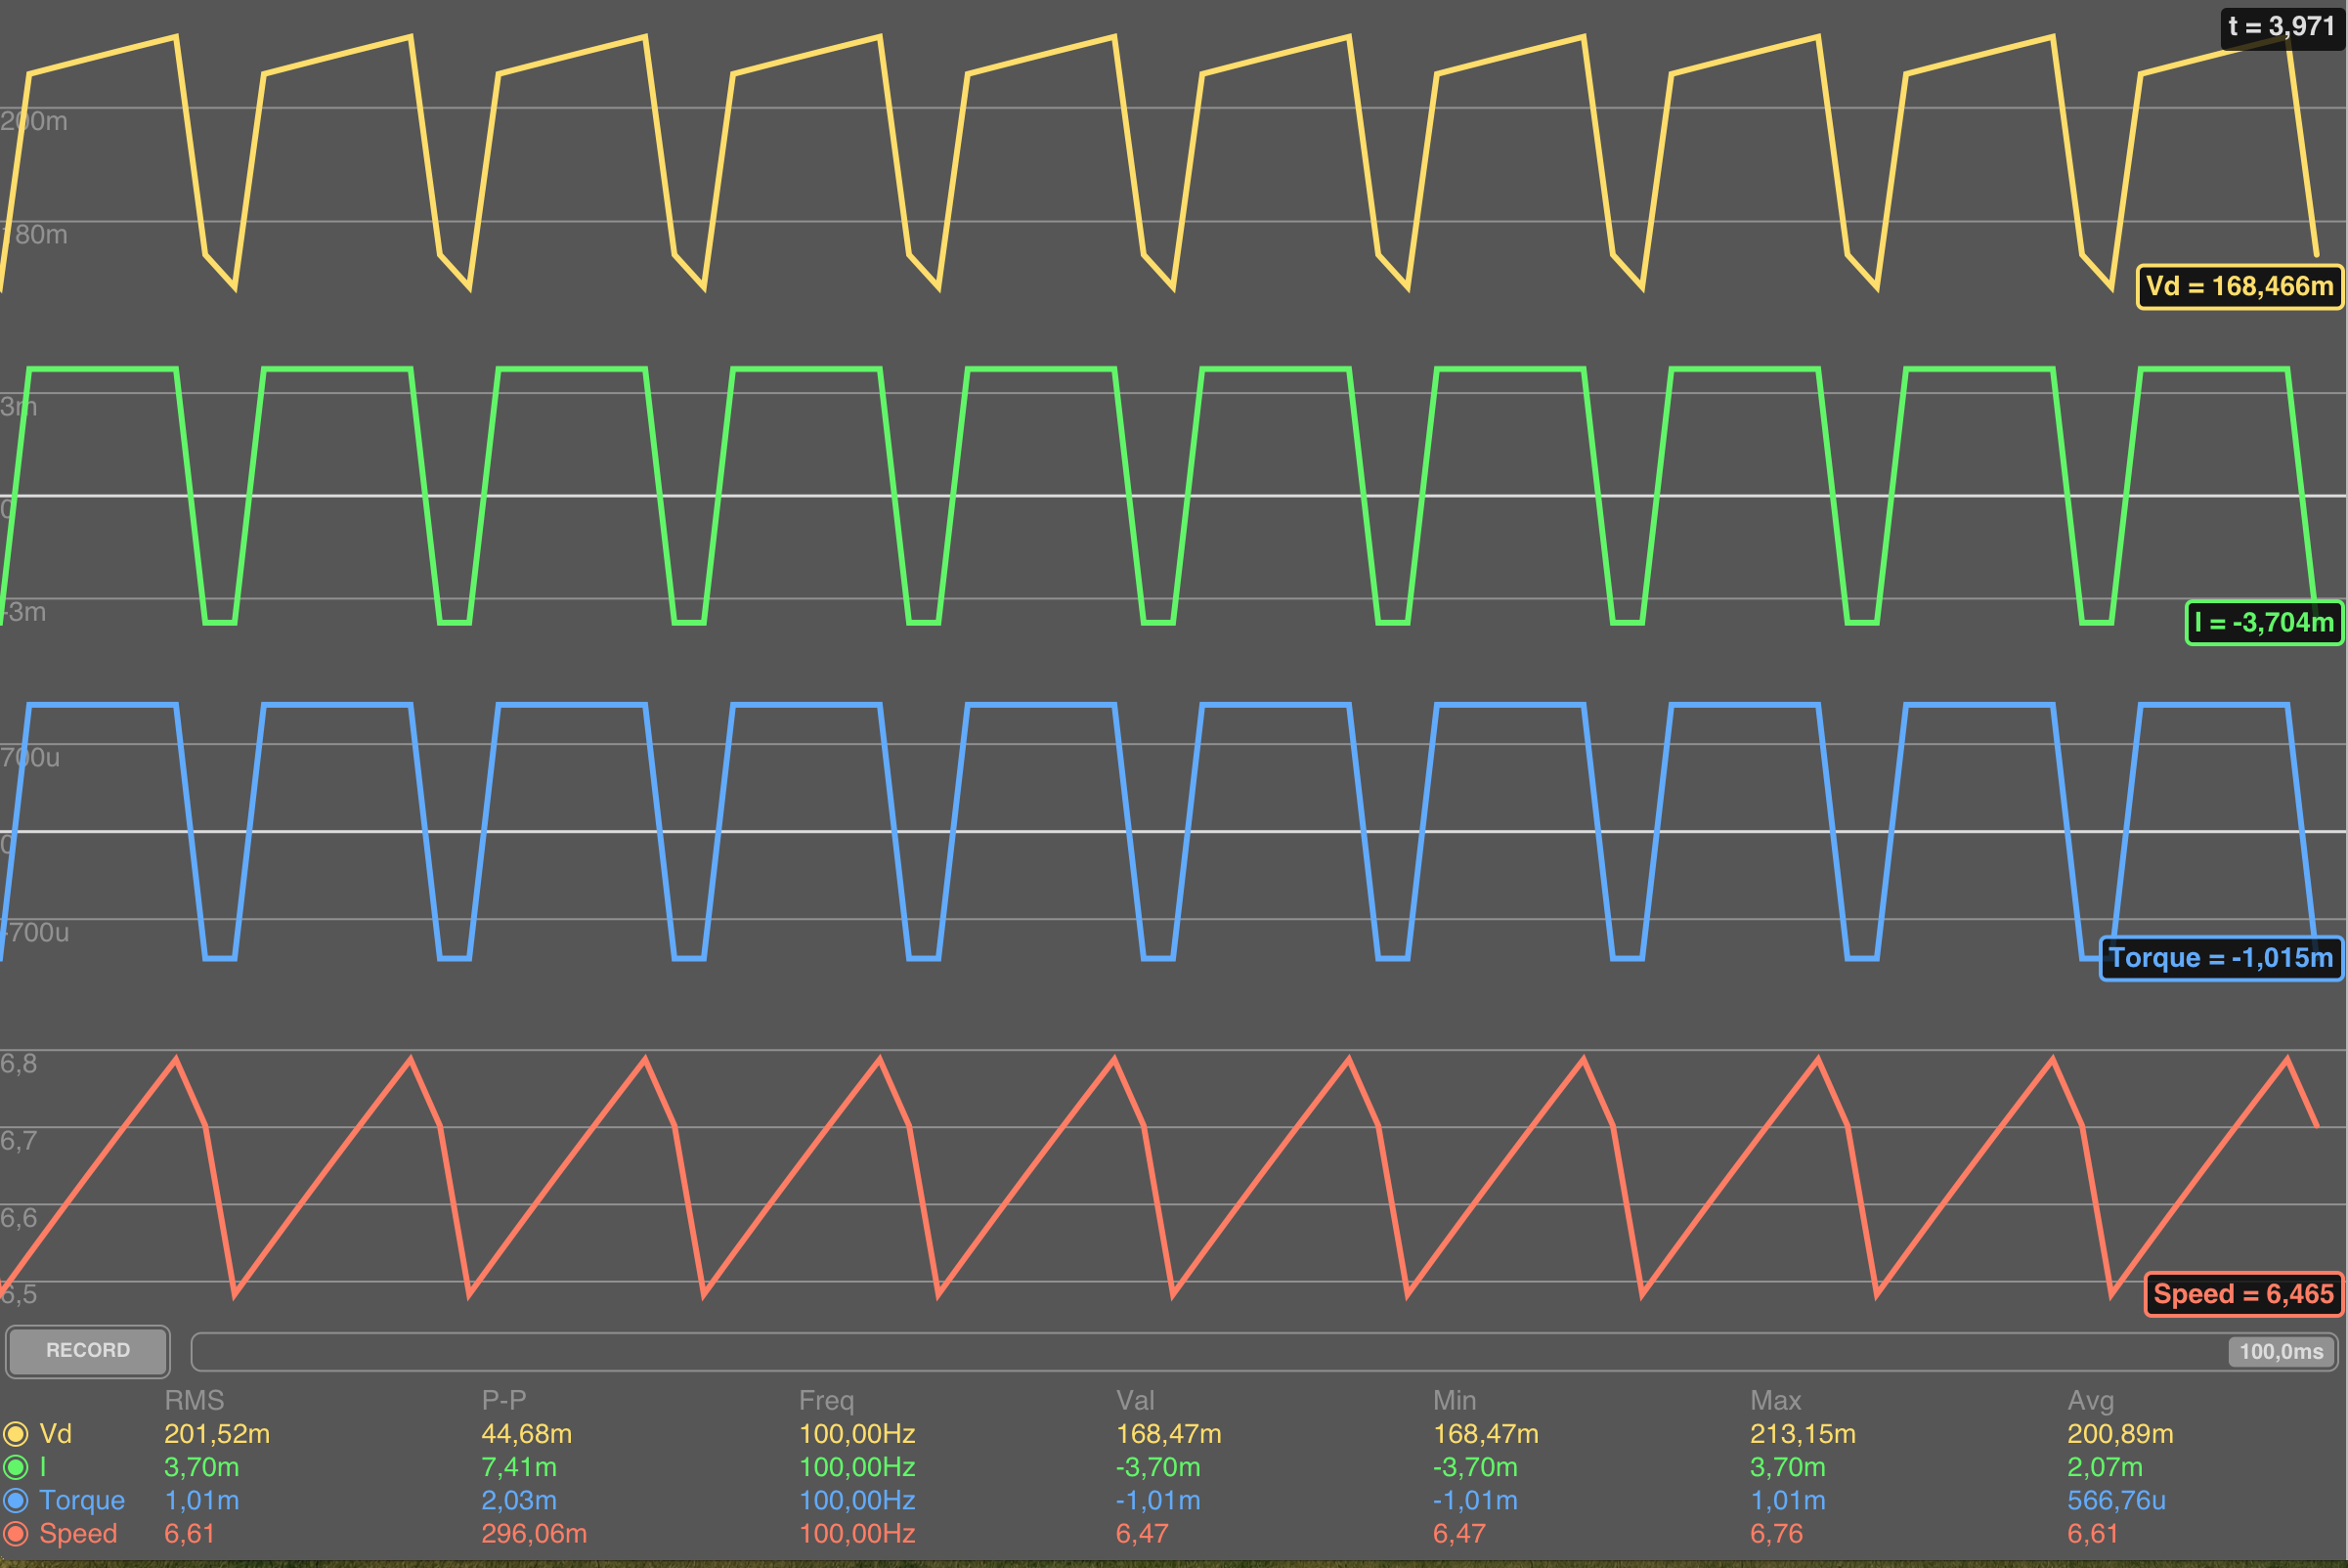
\includegraphics[width=1\textwidth]{simu7v}
	\caption{Simulation (boucle ouverte) avec une commande de 7V}
\end{figure}
\begin{figure}[H]
	\centering
	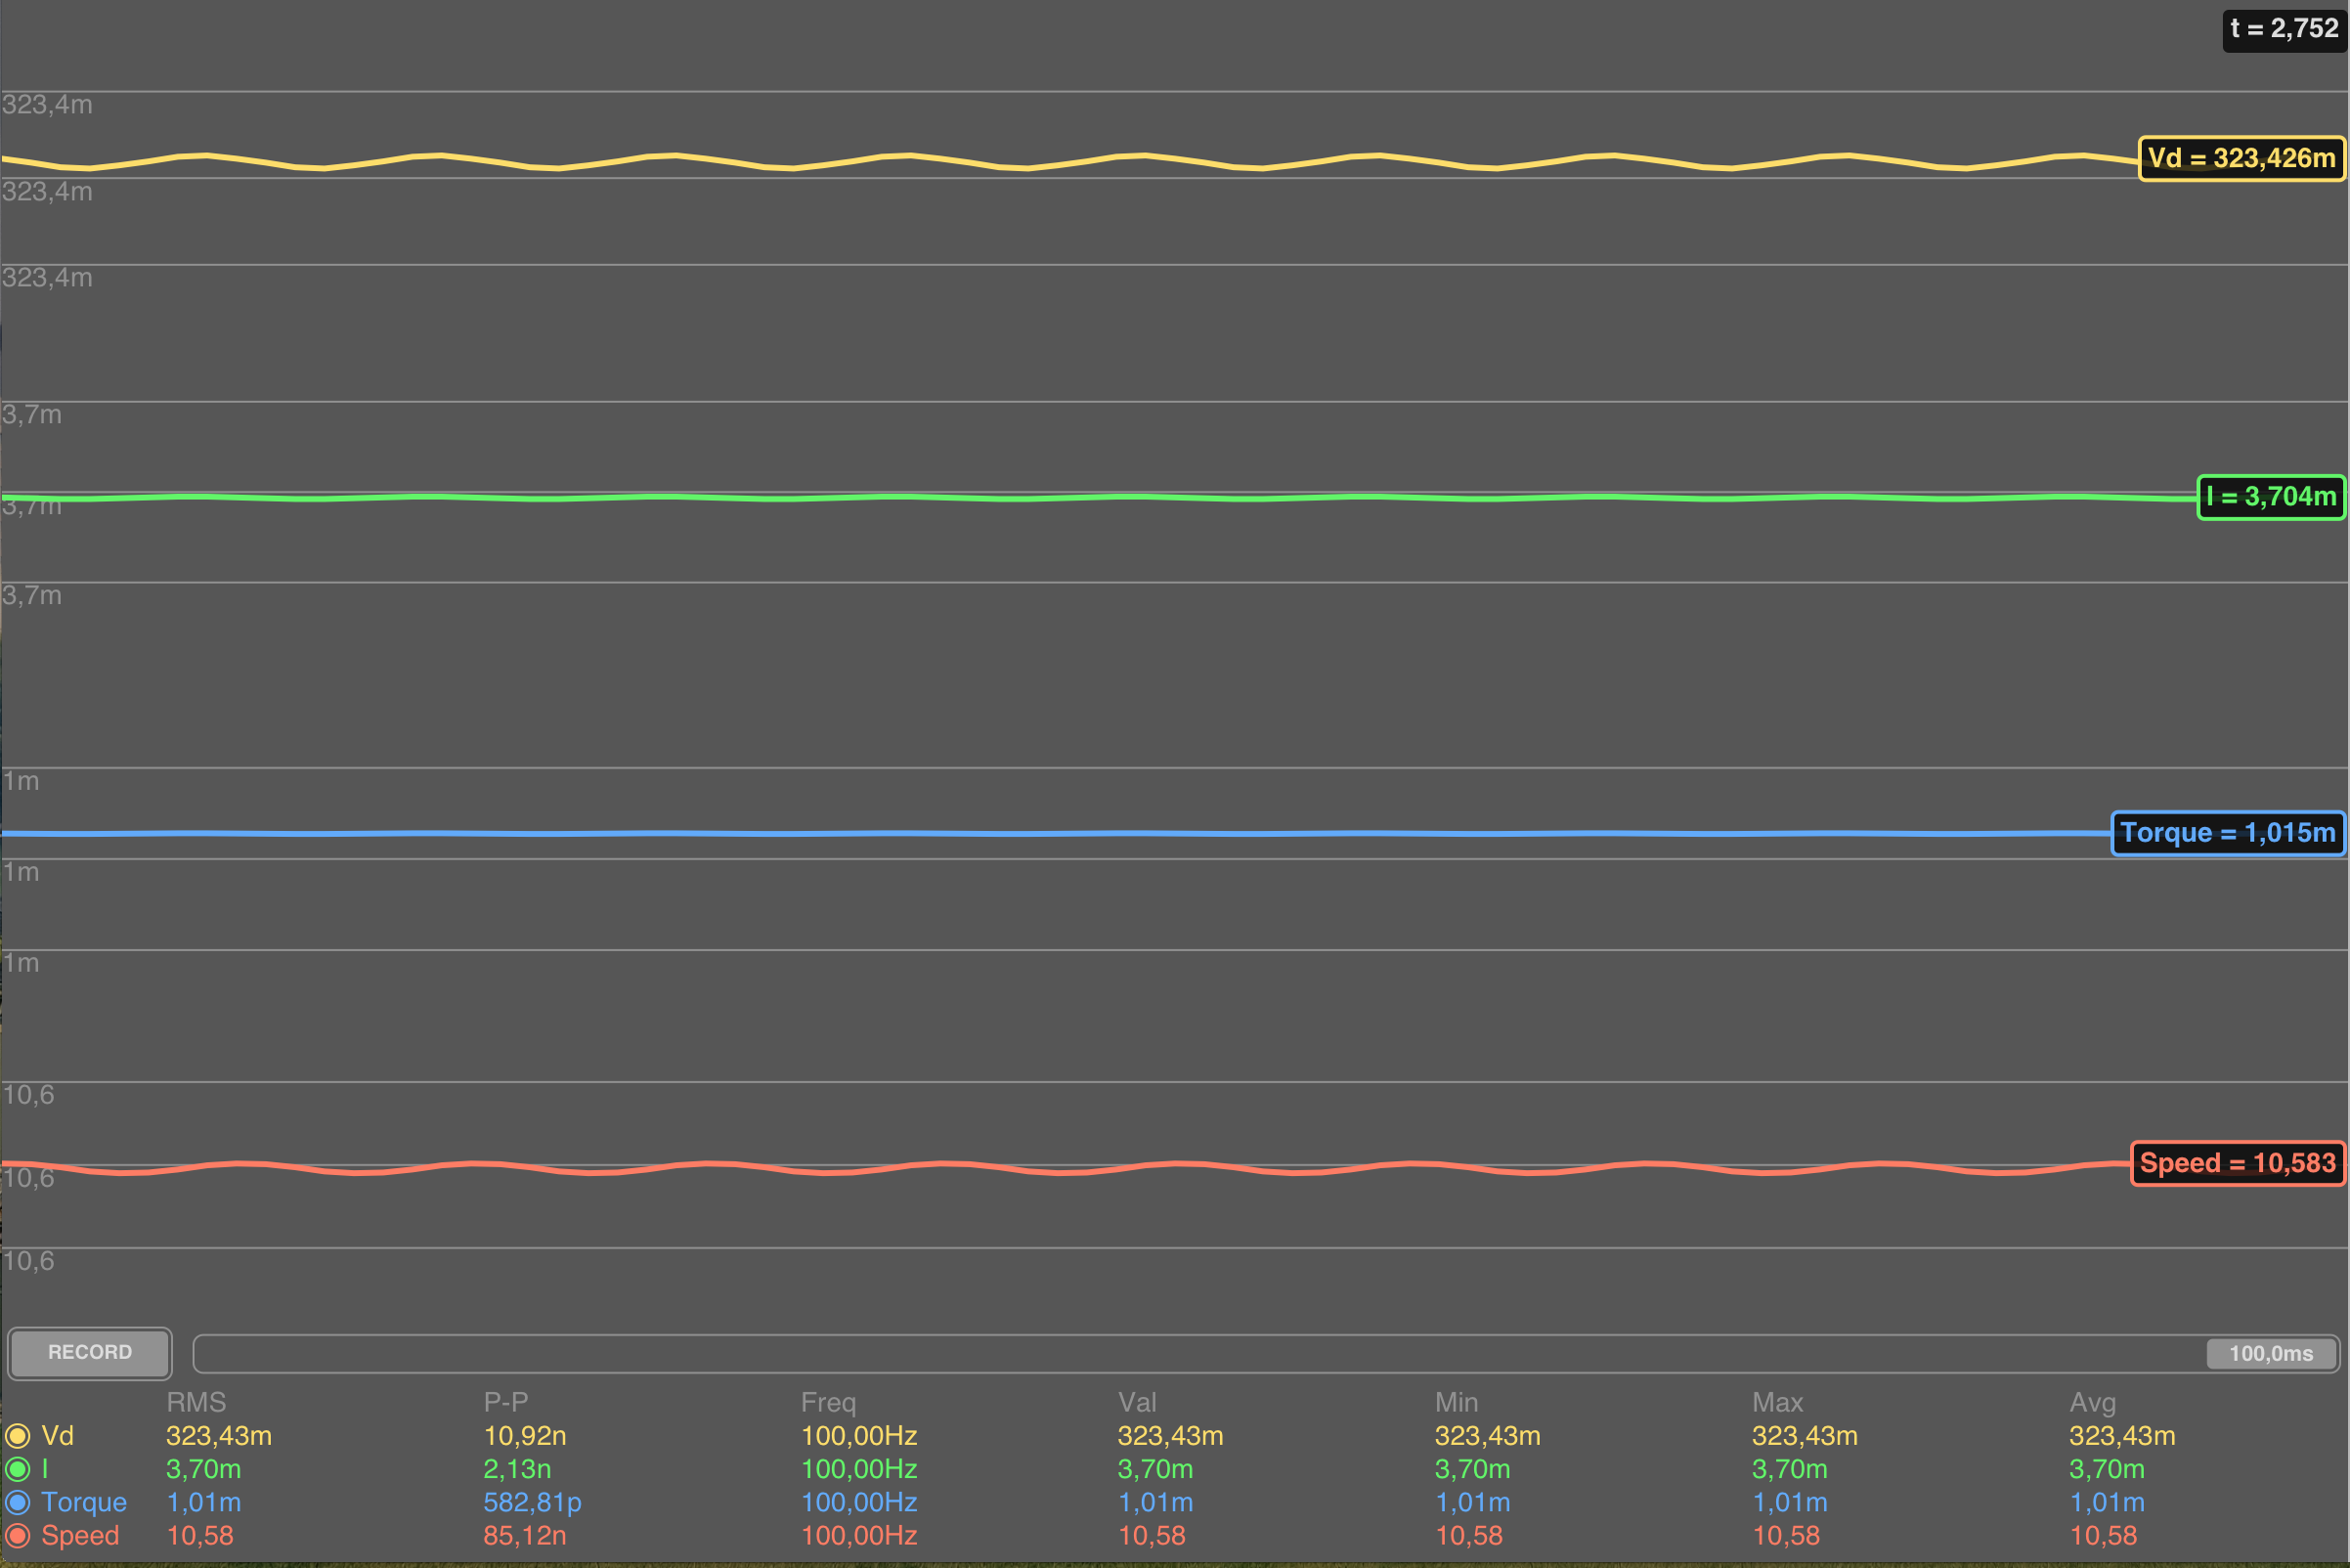
\includegraphics[width=1\textwidth]{simu15v}
	\caption{Simulation (boucle ouverte) avec une commande de 15V}
\end{figure}

\subsection{Circuit}

Après un certain nombre de problèmes de branchement, nous avons finalement réussi à faire fonctionner le circuit.

\begin{figure}[H]
  \centering
    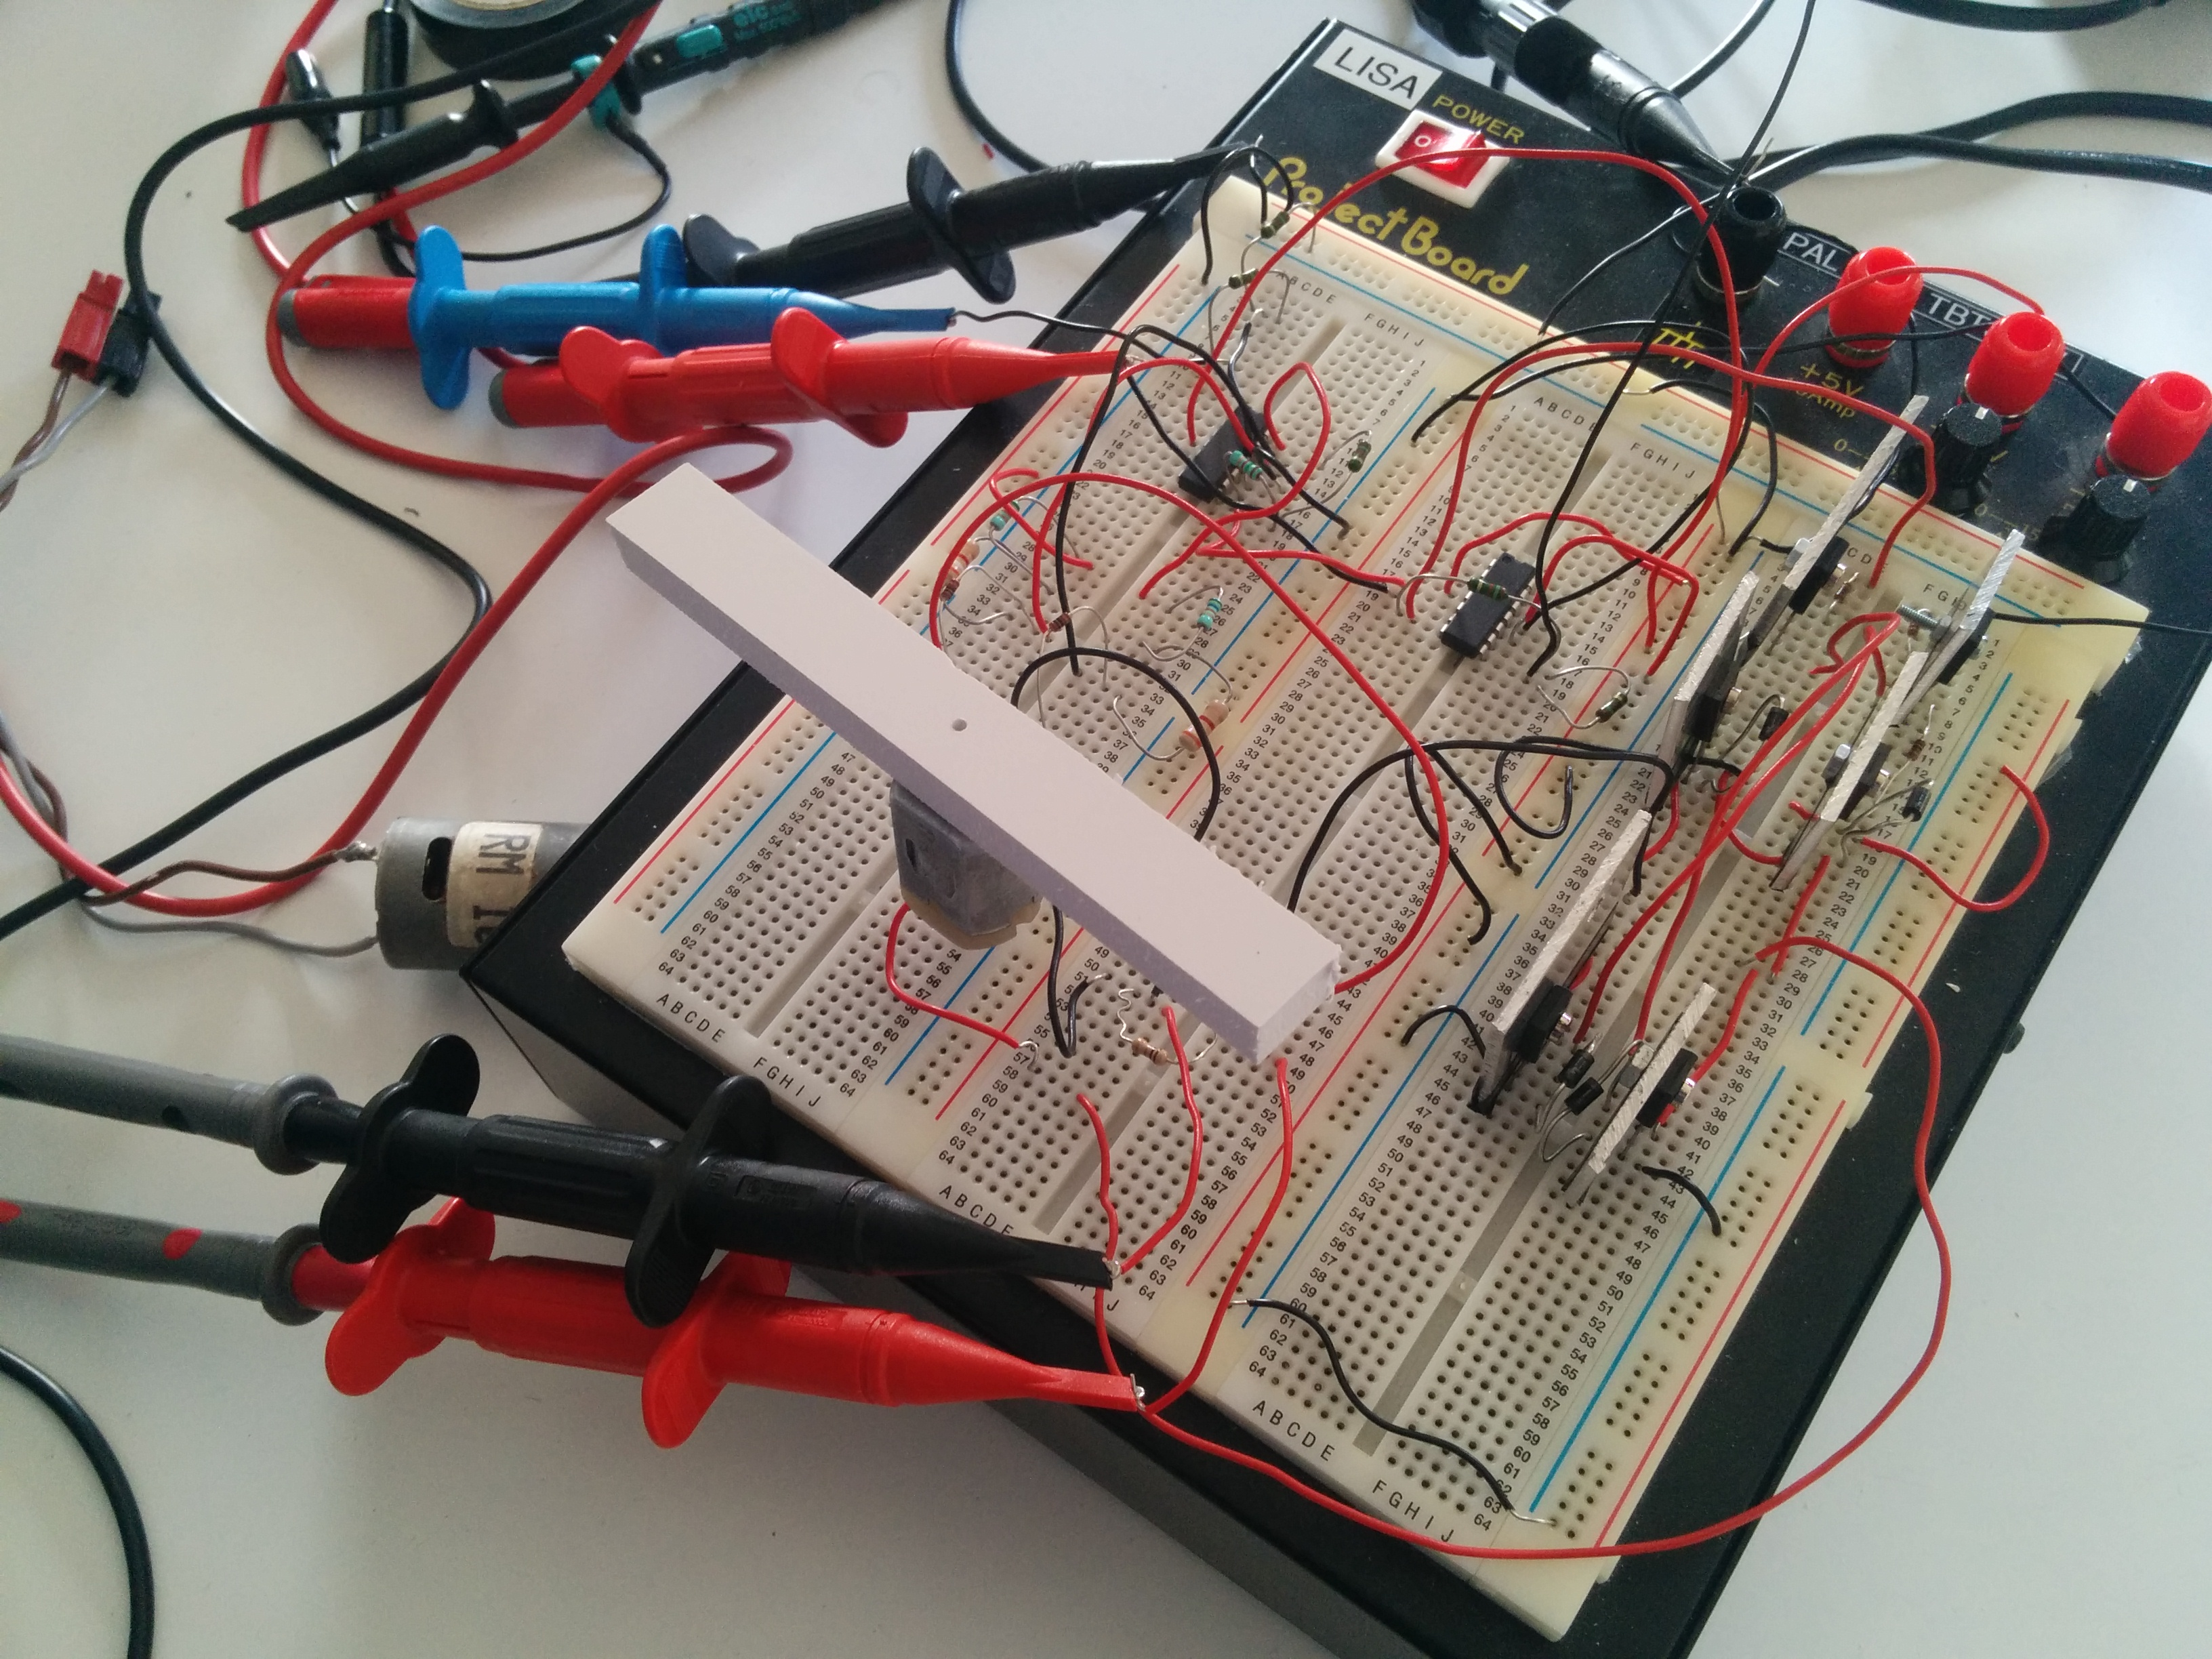
\includegraphics[width=1\textwidth]{circuit}
  \caption{Le circuit réalisé}
\end{figure}


\begin{figure}[H]
  \centering
    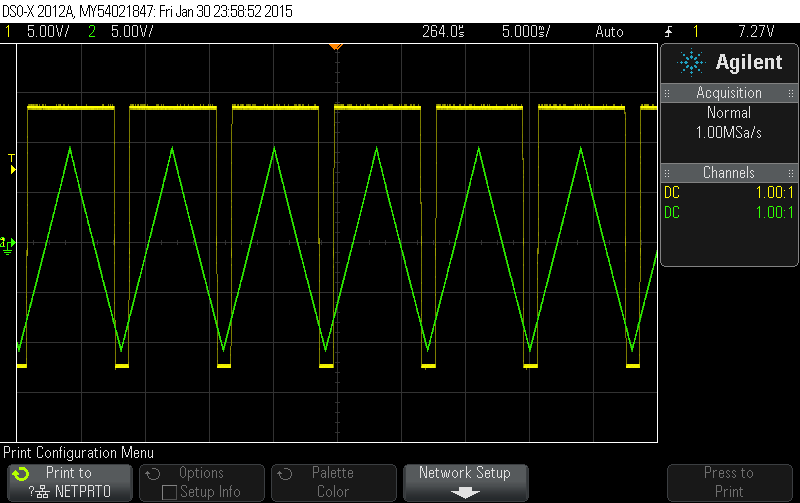
\includegraphics[width=1\textwidth]{scope_1}
  \caption{Entrée positive du pont en H}
\end{figure}

\begin{figure}[H]
  \centering
    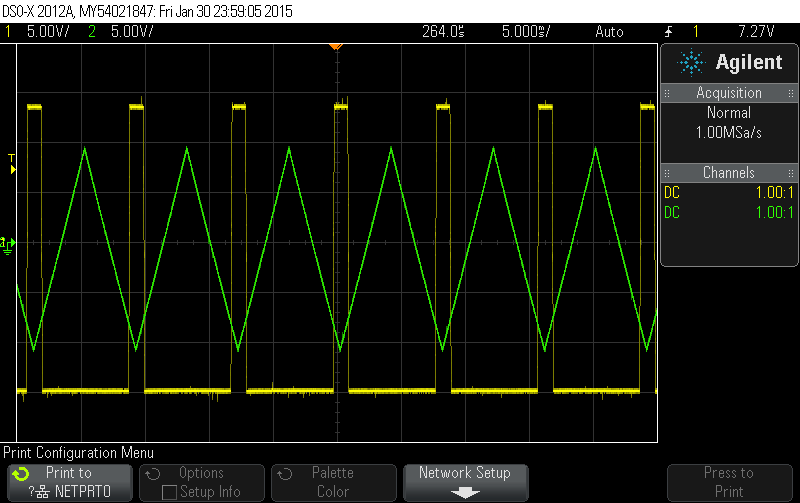
\includegraphics[width=1\textwidth]{scope_2}
  \caption{Entrée négative du pont en H}
\end{figure}

\begin{figure}[H]
  \centering
    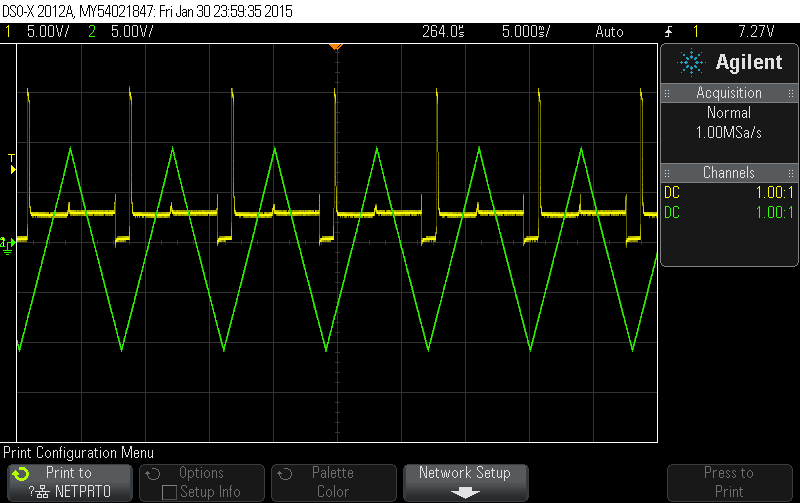
\includegraphics[width=1\textwidth]{scope_3}
  \caption{Tension aux bornes du moteur}
\end{figure}

\subsection{Résultats}

Le circuit fonctionne correctement en boucle ouverte. Il nous reste à rajouter une résistance de shunt au niveau du moteur afin de pouvoir injecter la mesure dans la boucle.


\end{document}